\documentclass[preprint,12pt]{elsarticle}

\usepackage[utf8]{inputenc}
\usepackage[T1]{fontenc}
\usepackage{lmodern}
\usepackage{amsmath,amssymb}
\usepackage{booktabs}
\usepackage{array}
\usepackage{graphicx}
\usepackage{tikz}
\usetikzlibrary{positioning,arrows.meta}
\usepackage{xcolor}
\usepackage{enumitem}
\usepackage[hidelinks]{hyperref}

\setlength{\emergencystretch}{2em}
\newcommand{\vcell}[2]{\begin{tabular}[t]{@{}c@{}}#1\#2\end{tabular}}

\begin{document}
\sloppy

\begin{frontmatter}

\title{Defending KG-RAG Against Knowledge Poisoning: Calibrated Path Filtering and Its Limits Under Adaptive Attack}

\author[iitp,lincoln]{Manish Nandish\corref{cor1}}
\ead{manish_25s21res58@iitp.ac.in}
\author[iitp]{Rajiv Misra}
\ead{rajivm@iitp.ac.in}
\author[lincoln]{Midhunchakkaravarthy Janarthanan}
\ead{midhun@lincoln.edu.my}
\cortext[cor1]{Corresponding author}

\affiliation[iitp]{organization={Department of Computer Science and Engineering, Indian Institute of Technology Patna},city={Patna},state={Bihar},country={India}}
\affiliation[lincoln]{organization={Lincoln University College},country={Malaysia}}

\begin{abstract}
Knowledge-graph retrieval-augmented generation (KG-RAG) answers questions from reasoning paths retrieved from a knowledge graph. Zhao et al. showed that a few fabricated triples completing plausible relation paths steer these systems to attacker-chosen answers, and evaluated no defence. We reproduce the attack with an open-weight generator (weaker: exact match falls 58\%, not 81\%) and study a defence that scores each retrieved path and removes suspicious ones before the LLM reads them. A gradient-boosted detector over 19 structural features, trained on 100 labelled development questions per attack type, with a conformal-risk-control removal threshold calibrated on 200 more, recovers 73\% [66, 81] of the gain of a perfect filter on WebQSP and 60\% [53, 68] on CWQ without retraining, when it filters every question. Text-RAG baselines do not help (RAGDefender adapted to KG paths lowers F1 by 12--19 points). Always-on filtering costs 5--6 F1 on clean graphs, so we gate it per question ($-$0.5 [$-$1.5, $+$0.4] F1). Against the attacker's best response among six attacks, three never seen in training, the gated filter raises worst-case F1 from 43.4 to 50.8 ($+$7.4 [$+$4.5, $+$9.9]); it recovers 33--64\% of a perfect filter's gain on the unseen families, against 76--82\% on the paper and adaptive attacks, and is level with no defence on the evasive attack. Full-precision (bf16) reruns agree with the 4-bit numbers to within 1.1 F1 on 1,328 questions. On a second system, GCR, the attack transfers but a perfect filter would add only $+$2.2 F1, because half of the damage is clean evidence overwritten by the inserted triples, and none of our detectors recovers even that.
\end{abstract}

\begin{highlights}
\item Structural path filter defends KG-RAG against poisoned triples
\item Conformal threshold removes suspicious paths with a tested risk bound
\item Question-level gate cuts the clean-data cost to 0.5 F1 points
\item Six attacks, three unseen in training; an evasive attacker still wins
\item On GCR the attack transfers but path filtering cannot recover the loss
\end{highlights}

\begin{keyword}
knowledge graph \sep retrieval-augmented generation \sep data poisoning \sep conformal risk control \sep adversarial robustness \sep question answering
\end{keyword}

\end{frontmatter}

\section{Introduction}
KG-RAG systems such as RoG, GCR, G-Retriever, SubgraphRAG and GNN-RAG answer knowledge-intensive questions by retrieving paths from a knowledge graph (KG) and letting an LLM reason over them. Their appeal is verifiability: the evidence is a path, not an opaque passage. That appeal makes tampering with the graph attractive. If the KG is assembled from third-party sources, updated by crowd contributors, or fed by extraction pipelines, an attacker can insert a few triples that make a wrong answer look as well supported as the right one~\cite{zhao2025}. On WebQSP the attack lowers RoG's F1 from about 70 to 38 in the original report, and we reproduce a 32\% relative F1 drop with a weaker generator (Section~\ref{sec:attack}).

The original attack paper proposes no defence. Text-RAG defences do not transfer directly: a poisoned triple is not a passage, there is no fluent adversarial text to flag, and the planted evidence is, by construction, locally consistent with the graph. Our central observation is that the \emph{structure} of planted evidence differs from natural evidence: to be retrieved, an attacker must complete a relation path to the wrong answer, and attackers who need robustness insert several chains per answer. These regularities (several paths ending at one rarely connected entity, low degree, few distinct incoming relations, little shared neighbourhood with the topic entity) are cheap to compute and can be learned from a small labelled development set. The detector fuses several such signals (end-entity degree, shared neighbourhood, relation variety and the number of paths converging on one entity) into one calibrated score per path, and the question-level gate fuses the path scores of a question into one decision.

\paragraph{Contributions.}
\begin{enumerate}[leftmargin=*,itemsep=2pt]
\item A defence pipeline for KG-RAG that scores each retrieved path and removes the suspicious ones before reasoning, evaluated end to end on WebQSP and CWQ with bootstrap confidence intervals (Sections~\ref{sec:method}, \ref{sec:main}).
\item A removal threshold calibrated with conformal risk control on development data only, used as the headline operating point, with an expected-risk guarantee that we test and show to fail under attack shift and on the large test sets (Section~\ref{sec:calib}).
\item A systematic adversarial evaluation: a decoy-adding adaptive attacker, an evasive one-chain attacker, attack-budget and seed variation. The relation-variety (rels) filter collapses under adaptivity, and a learned detector is only as good as the attack coverage of its training data (Section~\ref{sec:adaptive}). Results are also reported as a worst case over the attacks we built.
\item A question-level gate that removes the clean-data cost of the filter ($-$0.5 F1 for the recommended configuration) while keeping most of the worst-case gain (Sections~\ref{sec:adaptive}, \ref{sec:clean}).
\item A leave-attack-out evaluation on three attack families never seen in training, with a KG-embedding and an adapted RAGDefender baseline (Sections~\ref{sec:baselines}, \ref{sec:heldout}).
\item A negative result on a second system (GCR), where a perfect filter adds only $+$2.2 F1, and a MultiGraph ablation that isolates the cause of the oracle gap (Sections~\ref{sec:gcr}, \ref{sec:multigraph}).
\end{enumerate}

\section{Related Work}
\paragraph{KG-RAG.} RoG plans relation paths with a fine-tuned LLM and retrieves along them~\cite{luo2024rog}; GCR constrains decoding to paths in a KG-derived trie~\cite{luo2024gcr}; G-Retriever~\cite{he2024gretriever}, SubgraphRAG~\cite{li2025subgraphrag} and GNN-RAG~\cite{mavromatis2024} retrieve subgraphs with GNNs or scoring models.

\paragraph{Poisoning of RAG.} PoisonedRAG injects malicious passages into a text corpus~\cite{zou2024}. Zhao et al.~\cite{zhao2025} is, to our knowledge, the first study of triple-level poisoning of KG-RAG; it evaluates RoG, GCR, SubgraphRAG and G-Retriever and proposes no defence. Concurrent attacks (GragPoison, KEPo and others) target graphs built from text rather than curated KGs~\cite{fewwords2025,graphragfire2026,kepo2026}. Attacks on text-built GraphRAG keep appearing: LogicPoison swaps type-preserving entities~\cite{xiao2026logic}, Trigger-as-Entity plants backdoor entities~\cite{zheng2026trigger}, and Hop-Decayed Influence corrupts auxiliary index structures~\cite{park2026hop}; Oracle Poisoning corrupts a code knowledge graph that agents query at run time~\cite{kereopa2026}. Earlier work poisons knowledge-graph embedding models to change link predictions, not retrieved evidence~\cite{banerjee2021,you2023}. The authors of~\cite{zhao2025} later introduced ConflictQA and XoT~\cite{conflictqa2026}, which address conflicts between text and KG evidence at reasoning time, not injected KG triples.

\paragraph{Defences.} Text-RAG defences include RAGDefender~\cite{kim2025} (post-retrieval filtering of poisoned passages), TrustRAG-style clustering~\cite{zhou2025trustrag}, perplexity filters and LLM self-check; further passage-level defences include ReliabilityRAG~\cite{shen2025} and the filter of Edemacu et al.~\cite{edemacu2025}. For graph-based RAG, HoG-GRAG~\cite{noughabi2026} repairs subgraphs of \emph{text-built} GraphRAG hop by hop, and DMI-RAG~\cite{fei2026} fine-tunes the LLM with preference and graph-contrastive objectives against graph noise and KG poisoning (HotpotQA and two further datasets; available only as a poster abstract). CS-RAG~\cite{ma2026csrag} makes GraphRAG robust to spurious or missing edges in LLM-built graphs but does not model an adversary. A distinct TrustRAG for KG-RAG~\cite{li2026} scores edge-level support and contradiction on a medical KG and has no attack evaluation. We differ in target (Freebase KG-RAG with RoG/GCR retrieval), mechanism (learned path scoring and calibrated removal, no LLM training) and evaluation (end to end under adaptive attackers). RAGDefender is adapted to KG paths and evaluated in Section~\ref{sec:baselines}; HoG-GRAG, designed for text-built GraphRAG, was not ported. As of 10 October 2026 we found no published defence for triple-level poisoning of KG-RAG on curated knowledge graphs: keyword searches, the works citing Zhao et al.\ in OpenAlex (10) and Semantic Scholar (5), and the full texts we downloaded turned up only the attacks and text-RAG defences above.

\paragraph{KG error detection.} Triple-level error detectors such as SIT-KGED~\cite{sitkged2026}, LKED~\cite{lked2026} and PTrustE~\cite{ptruste2022} (which scores triples by path trustworthiness) classify static KG triples; they are not designed for adversarial, path-completing insertions and operate before retrieval.

\paragraph{Risk control.} Conformal risk control~\cite{angelopoulos2024} and Learn-then-Test~\cite{angelopoulos2021} calibrate a threshold so that an expected loss is bounded. We use the former for the removal level. Calibration for KG-RAG has so far addressed answer confidence (Ca2KG~\cite{ren2026ca2kg}), not the removal of retrieved evidence under attack.

\section{Problem and Threat Model}\label{sec:threat}
\paragraph{Setting.} A question $q$ with topic entities and a KG subgraph $G$ (about 4{,}300 triples per question in the RoG-WebQSP/CWQ release). A retriever returns a set of paths $P(q,G)$; a reasoner LLM answers from $P$. A defence is a function $\Phi$ that removes paths from $P$ before reasoning.

\paragraph{Attacker (black-box, following Zhao et al.).} For each question an LLM proposes $N$ plausible wrong answers; for each, $K$ triples are inserted that complete a relation path from the topic entity to the wrong answer, using only existing entities and relations. The attacker does not see gold answers. Because it does not see them either, its wrong answers are not filtered against them: in 13.4\% of the WebQSP-500 questions (12.9\% of the 1,328 and 9.3\% of the CWQ questions) at least one wrong answer coincides with a gold answer, and 6.8\% of the poisoned paths end in a gold answer. The planted-answer rate counts such answers as planted and the oracle removes their paths. Setting these 67 questions aside leaves the share of the oracle gain recovered by D unchanged (76.1\% against 76.2\%) and raises the damage of the attack from 21.8 to 23.4 F1. We use $N=5$, $K=4$ as in the original, with Qwen2.5-7B-Instruct as the generator instead of GPT-4, a deviation that likely weakens the attack (Section~\ref{sec:attack}). The data-availability statement of the original paper points only to the public benchmarks and the RoG model, so their poisoned graphs and attack code are not available to reuse.

Figure~\ref{fig:attack} illustrates the attack and the signature the scorer uses.
\begin{figure}[tbp]
\centering
\resizebox{0.95\textwidth}{!}{%
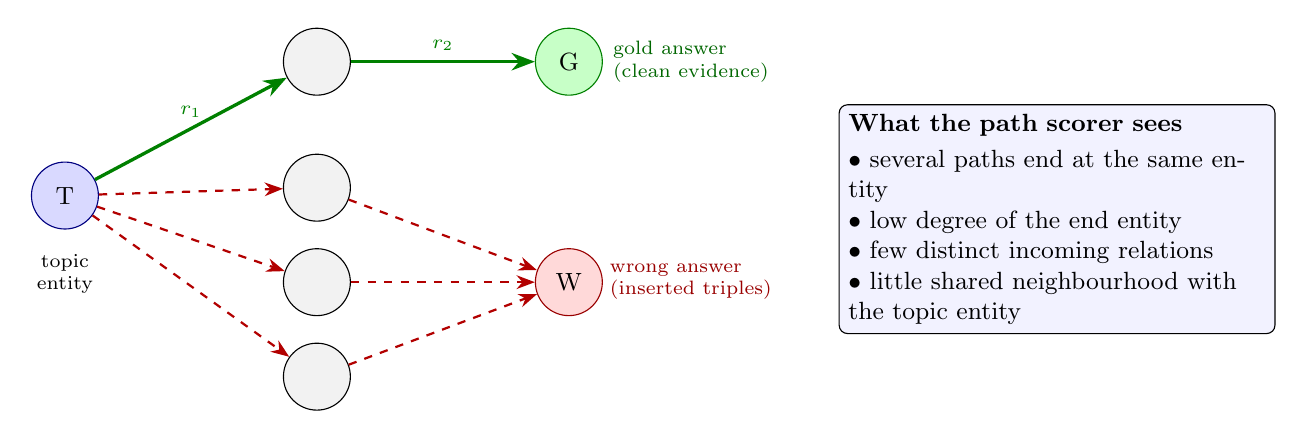
\begin{tikzpicture}[>=Stealth, font=\small,
  ent/.style={circle, draw, minimum size=0.85cm, inner sep=1pt},
  topic/.style={ent, fill=blue!15, draw=blue!50!black},
  gold/.style={ent, fill=green!22, draw=green!50!black},
  wrong/.style={ent, fill=red!15, draw=red!60!black},
  mid/.style={ent, fill=gray!10}]
\node[topic] (T) at (0,0) {T};
\node[mid] (A) at (3.2,1.7) {};
\node[gold] (G) at (6.4,1.7) {G};
\node[mid] (B1) at (3.2,0.1) {};
\node[mid] (B2) at (3.2,-1.1) {};
\node[mid] (B3) at (3.2,-2.3) {};
\node[wrong] (W) at (6.4,-1.1) {W};
\draw[->, green!50!black, very thick] (T) -- node[above, font=\scriptsize] {$r_1$} (A);
\draw[->, green!50!black, very thick] (A) -- node[above, font=\scriptsize] {$r_2$} (G);
\foreach \b in {B1,B2,B3}{
  \draw[->, red!70!black, dashed, thick] (T) -- (\b);
  \draw[->, red!70!black, dashed, thick] (\b) -- (W);}
\node[align=left, font=\scriptsize, green!40!black] at (7.95,1.7) {gold answer\\ (clean evidence)};
\node[align=left, font=\scriptsize, red!60!black] at (7.95,-1.1) {wrong answer\\ (inserted triples)};
\node[align=center, font=\scriptsize] at (0,-1.0) {topic\\ entity};
\node[draw, rounded corners=3pt, fill=blue!5, align=left, text width=5.3cm, font=\small] at (12.6,-0.3)
  {\textbf{What the path scorer sees}\\[2pt]
   $\bullet$ several paths end at the same entity\\
   $\bullet$ low degree of the end entity\\
   $\bullet$ few distinct incoming relations\\
   $\bullet$ little shared neighbourhood with the topic entity};
\end{tikzpicture}}
\caption{The attack and its signature. The topic entity T has clean evidence (green) leading to the gold answer G. The attacker inserts triples (red, dashed) that complete several relation paths from T to a wrong answer W, using only existing entities and relations. Repeated chains into one rarely connected entity are what the learned detector picks up.}
\label{fig:attack}
\end{figure}

\paragraph{Adaptive variants (ours).} \emph{Decoys}: $m=8$ extra triples per wrong answer that mimic ordinary neighbourhood structure. \emph{Evasive}: $K=1$ (no repeated-chain signature) plus 12 decoys per answer placed next to the topic entity's neighbours. Budget variants $K=1$ and $K=8$. A stronger budget $N=10$, $K=8$ is evaluated in Section~\ref{sec:budget}. Three held-out families (Section~\ref{sec:heldout}): \emph{profile-copy} (the paper's chains plus decoys that copy the degree and relation profile of a real endpoint of the clean paths), \emph{bridge} (full-length chains made only of inserted triples through random bridge entities) and \emph{spread} (the number of chains per wrong answer varies from 1 to 8, total budget fixed at 20). None uses the gold answers.

\paragraph{Defender knowledge.} The defender has a small labelled development set (300 WebQSP questions, indices 1000:1300) with known inserted triples, standing in for a red-team exercise on the defender's own graph. The defender does not know the test attacker's parameters unless stated (``attack-aware'').

\paragraph{Goal.} Maximise answer F1 under attack while keeping the loss on clean graphs small and bounding the probability of removing all correct evidence.

\section{Method}\label{sec:method}
Figure~\ref{fig:overview} gives an overview.
\begin{figure}[tbp]
\centering
\resizebox{\textwidth}{!}{%
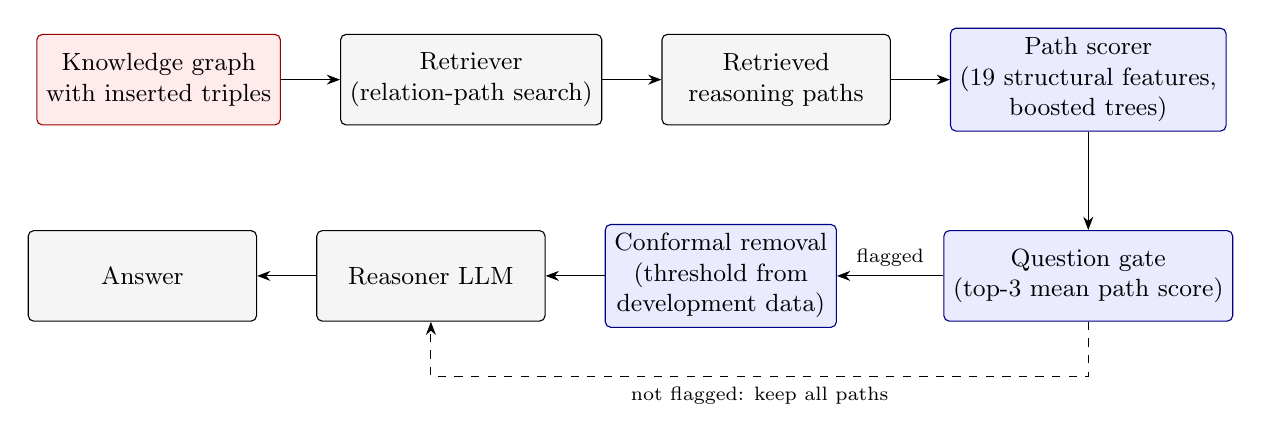
\begin{tikzpicture}[>=Stealth, node distance=0.55cm and 0.75cm,
  box/.style={draw, rounded corners=2pt, align=center, minimum height=1.15cm, minimum width=2.9cm, font=\small, fill=gray!8},
  att/.style={box, draw=red!60!black, fill=red!8},
  def/.style={box, draw=blue!50!black, fill=blue!8}]
\node[att] (kg) {Knowledge graph\\ with inserted triples};
\node[box, right=of kg] (ret) {Retriever\\ (relation-path search)};
\node[box, right=of ret] (paths) {Retrieved\\ reasoning paths};
\node[def, right=of paths] (score) {Path scorer\\ (19 structural features,\\ boosted trees)};
\node[def, below=1.25cm of score] (gate) {Question gate\\ (top-3 mean path score)};
\node[def, left=1.35cm of gate] (crc) {Conformal removal\\ (threshold from\\ development data)};
\node[box, left=of crc] (llm) {Reasoner LLM};
\node[box, left=of llm] (ans) {Answer};
\draw[->] (kg) -- (ret);
\draw[->] (ret) -- (paths);
\draw[->] (paths) -- (score);
\draw[->] (score) -- (gate);
\draw[->] (gate) -- node[above, font=\scriptsize, align=center] {flagged} (crc);
\draw[->] (crc) -- (llm);
\draw[->] (llm) -- (ans);
\draw[->, dashed] (gate.south) -- ++(0,-0.7) -| node[pos=0.25, below, font=\scriptsize] {not flagged: keep all paths} (llm.south);
\end{tikzpicture}}
\caption{The defence sits between retrieval and reasoning. Every retrieved path is scored; a question-level gate decides whether a question looks attacked, and only then are paths whose score exceeds the conformal threshold removed before the reasoner reads them.}
\label{fig:overview}
\end{figure}

\paragraph{Path scoring.} For every retrieved path we compute, in the question's own subgraph, seven structural values: the degree of the end entity, the minimum degree of the entities on the path, the number of distinct relation types incident to the end entity, and, for the last edge and as a minimum over the path's edges, the number of neighbours shared by the edge's two endpoints and their Jaccard overlap. The seven values are log-scaled and also z-scored within the question (14 features). Five further features describe the path and its question: path length, the number of retrieved paths that end in the same entity (raw and divided by the number of paths), the share of retrieved paths with the same last relation, and the number of retrieved paths. That makes 19 features (\texttt{kgrag/learned.py}).

\paragraph{Detector.} A HistGradientBoosting classifier (200 iterations, learning rate 0.08, depth 5) is trained on the development paths; the label is whether the path contains an inserted triple (strict label for the rows marked strict in Section~\ref{sec:setup}, original label for the others). Permutation importance shows that the count features dominate; an evasive attacker therefore targets exactly them (Section~\ref{sec:adaptive}).

\paragraph{Removal level.} A path is removed if its score exceeds a threshold. We set the threshold from out-of-fold development scores so that a target fraction (the false-positive rate, FPR) of clean development paths is removed. At 10\% FPR the filter deletes all clean gold evidence in 18\% (original labels) to 21\% (strict labels) of the questions that have any, so we evaluate 2\%, 5\% and 10\% and recommend 2--5\%. \emph{The 2\% operating point was chosen after inspecting the first 500 test questions of WebQSP; we report all levels, and the full 1{,}328-question set contains 828 questions not used for that choice (same 61.2 F1). The headline results use the conformal threshold, which is selected on development data only.}

\paragraph{Conformal calibration.} The loss is 1 if \emph{all} clean gold-supporting paths of a question are removed, else 0. We choose the smallest threshold whose adjusted empirical risk $\frac{n}{n+1}\hat R + \frac{1}{n+1}$ is at most $\alpha$ on a calibration split, giving risk at most $\alpha$ in expectation under exchangeability of calibration and test questions. We also report realised single-split risk and behaviour under attack shift. Calibration is a clean split: the detector is trained on the first 100 questions of each development split and the threshold is calibrated on the remaining 200, never on the detector's own training questions, so calibration and test questions are exchangeable (the fixed-FPR levels, by contrast, use out-of-fold scores and carry no formal guarantee).

\paragraph{Question-level gate.} A question is scored by the mean of its top-3 path scores from a detector trained on poisoned plus clean development questions; it is filtered only if the score reaches a threshold chosen so that 5\% of held-out clean development questions are flagged (5.2\% in practice, because of ties). Every gate in this paper uses 5\%. On the clean WebQSP-500 test questions the gate flagged 6.8\% (detector C) and 6.4\% (detector D); a question with fewer than three paths is scored by the mean of the paths it has, and a question without any path is never flagged. It is implemented in \texttt{kgrag/gate.py}; the end-to-end results are in Section~\ref{sec:clean}.

\section{Experimental Setup}\label{sec:setup}
\paragraph{Data.} WebQSP (1{,}628 test questions) and CWQ (3{,}531) from \texttt{rmanluo/RoG-webqsp} and \texttt{rmanluo/RoG-cwq}. WebQSP: development 1000:1300; main test set 0:500; full test 0:1000 plus 1300:1628 (1{,}328 questions). CWQ: development 500:800; full test is the remaining 3{,}231 questions. The WebQSP development questions are taken from the test split (RoG was fine-tuned on the training split), which leaves a non-standard 1{,}328-question test set. The detector is trained on WebQSP development data only, so CWQ is cross-dataset transfer; the CWQ development questions were used only for a CWQ-trained detector variant, which did worse on CWQ-500 than the WebQSP-trained one (F1 gain at 2\% FPR $+$4.9 [$+$0.6, $+$9.4] versus $+$11.1 [$+$7.2, $+$15.0]).

\paragraph{Systems.} RoG (Llama-2-7B based, 4-bit NormalFloat (nf4) quantisation on a 16~GB GPU; relation-path BFS retrieval). A second reasoner: Qwen2.5-7B-Instruct reading RoG's paths. GCR (attack and defence) in Section~\ref{sec:gcr}; full-precision (bf16) confirmation in Section~\ref{sec:bf16}.

\paragraph{Metrics.} Hit (any gold answer in the prediction), F1, precision and recall as in the RoG repository; \emph{planted-answer rate} (A-Precision in the logs) is the share of a question's predicted answers that are among the attacker's wrong answers, averaged over questions; a question has a \emph{planted top-1} when its first predicted answer is a wrong answer (A-Hit@1). Hit counts a question as correct when any gold answer occurs in the prediction; EM (exact match) requires the set of predicted answers to equal the gold set after normalisation. F1, Hit, precision and recall come from one scoring function (\texttt{rog.score}) for RoG, the Qwen reasoner and GCR, and a question left without any retained path gets an empty prediction and scores 0. 95\% intervals are percentile bootstrap over questions (2{,}000 resamples, seed 0); differences against ``none'' are paired. Worst-case gains use the difference of the observed worst cases as point estimate and a basic bootstrap interval (5{,}000 resamples, seed 0, the minimum over attacks taken inside each resample).

\paragraph{Baselines.} Random, degree, relation variety (``rels''), TrustRAG-style embedding clustering (``similarity''), perplexity filter, LLM self-check (``verify''), and an oracle that removes exactly the inserted paths (under the strict label below). It is close to, but not identical with, the clean-graph run: in 62 of 500 WebQSP questions the paths the oracle keeps differ from the clean graph's, and there the oracle scores 63.4 against 81.3 (strict labels), a gap that comes from RoG's graph representation: it stores one relation per entity pair (a networkx Graph), so an inserted triple on an existing pair overwrites the clean relation and removing the inserted path cannot restore it (53 of those 62 questions have a clean path missing; our retrieval has no path cap). A MultiGraph ablation that keeps parallel edges closes the gap completely (oracle 74.6 against clean 74.6, Section~\ref{sec:multigraph}). Thresholds differ between the baselines (Section 6.3): similarity, perplexity, self-check and rels remove the paths above the score at which 10\% of clean development paths are removed, the learned detector (headline row) and TransE use 2\%, and RAGDefender is a removal rule that deletes its own estimate of the number of adversarial paths per question and has no threshold. At the same 10\% level the learned detector reaches 54.2 on the paper attack (rels: 54.4), so the lead of the learned detector in Section 6.3 comes from its stricter 2\% operating point, not from a higher score at equal removal.

\paragraph{Poisoned-path label.} A retrieved path is labelled poisoned (strict) only if it uses an inserted triple that is not already in the clean graph in either orientation; otherwise a reversed duplicate of a clean triple would mark a clean path as poisoned. The strict label changes 0.94\% of paths (166 of 17,703 paths on the WebQSP-500 paper-attack test set). The oracle and the always-on conformal filter with the paper-attack detector (A) are run with strict labels on WebQSP-1328 and CWQ-3231, and C, D and the oracle on WebQSP-500 (known attacks and held-out families), in both the training splits and the test paths; A's WebQSP-500 row in Section~\ref{sec:adaptive} keeps the original labels. Against the original labelling, F1 moves by at most 1.8 on any strict rerun and no conclusion changes; the largest shifts are the strict oracle on CWQ ($+$1.8 [$+$1.2, $+$2.3]), C on the evasive attack ($-$1.7 [$-$2.7, $-$0.7]) and A on WebQSP-500 ($+$1.6 [$-$0.1, $+$3.4]).

\paragraph{Disjointness.} Detector training and conformal calibration use development questions only; no test question is used for fitting. Configuration D (gate, conformal threshold, mixed detector) was selected after we saw the WebQSP-500 results on the known attacks; the held-out families (Section~\ref{sec:heldout}), where D is applied unchanged, are therefore its untouched evaluation, whereas the CWQ gate (Section~\ref{sec:cwqkge}) uses the paper-detector variant C.

\section{Results}
\subsection{Reproducing the attack}\label{sec:attack}
On WebQSP-500 with RoG, Hit falls from 83.2 to 78.0 ($-$6\% relative) and F1 from 67.7 to 45.9 ($-$32\%); the attacker's wrong answers make up 47.7\% of the predicted answers (the planted-answer rate; at least one wrong answer appears in 71.2\% of the outputs). Zhao et al.\ (Table 3 of the published version; GPT-4 generator, $N=5$, $K=4$) report for RoG on WebQSP F1 70.34 $\rightarrow$ 38.06 ($-$46\%), EM 45.76 $\rightarrow$ 8.85 ($-$81\%), Hits@1 79.61 $\rightarrow$ 48.46 ($-$39\%) and Hit 85.87 $\rightarrow$ 75.61 ($-$12\%). On the same metrics our WebQSP-500 numbers are EM 43.0 $\rightarrow$ 18.2 ($-$58\%), F1 $-$32\% and Hit $-$6\%; our clean EM (43.0) is close to theirs (45.76), which supports the reproduction of the clean system. Their figures are on the full WebQSP test set and ours on 500 questions with a different generator, so the comparison is indicative. \textbf{Our attack is weaker than the original on every metric we can compare.} Plausible causes are a 7B open generator instead of GPT-4 (less convincing wrong answers), 4-bit weights, and implementation differences in grounding. This makes the defence's task easier, so Section~\ref{sec:budget} repeats the evaluation with a larger budget ($N=10$, $K=8$): F1 then falls 38\% and Hit 10\% relative to clean, close to the original's Hit drop ($-$12\%). Its EM drop stays at $-$58\% (18.0 against 18.2), in line with their observation that increasing $K$ beyond 4 gives diminishing returns (our budget run raises $N$ as well as $K$, so we cannot attribute the plateau to $K$ alone).

\subsection{Main result}\label{sec:main}
\begin{table}[tbp]
\centering\small
\resizebox{\textwidth}{!}{%
\begin{tabular}{@{}lrrrrrr@{}}
\toprule
Setting (RoG, 4-bit) & $n$ & Clean & None & Learned @2\% & Conformal $\alpha{=}0.05$ & Oracle \\
\midrule
WebQSP, paper attack & 1{,}328 & 67.2 & 45.3 [43.3, 47.1] & 61.2 [59.0, 63.2] & \textbf{60.1} [57.9, 62.4] & 65.6 [63.4, 67.8] \\
CWQ, paper attack (detector from WebQSP) & 3{,}231 & 48.9 [47.2, 50.5] & 35.3 [33.8, 36.8] & 43.6 [41.9, 45.1] & \textbf{43.2} [41.6, 44.8] & 48.4 [46.7, 50.0] \\
\bottomrule
\end{tabular}}
\caption{F1 (\%) with 95\% bootstrap intervals under the paper attack (WebQSP-1328 and CWQ-3231; RoG, 4-bit). The conformal column is the always-on filter with the paper-attack detector (configuration A). Conformal and oracle columns use strict labels; the learned @2\% column keeps the original labelling.}
\end{table}
The gain over no defence with the conformal threshold is $+$14.9 [$+$12.8, $+$17.0] on WebQSP and $+$7.9 [$+$6.5, $+$9.3] on CWQ (fixed 2\% level: $+$15.9 [$+$13.8, $+$17.9] and $+$8.3 [$+$6.8, $+$9.8]). The share of the oracle's gain recovered (paired bootstrap) is, with the conformal threshold (chosen on development data only), \textbf{73.2\% [65.7, 80.5]} on WebQSP and \textbf{60.2\% [52.5, 67.8]} on CWQ (the strict oracle is stronger on CWQ, $+$13.1 against $+$11.4 under the original labelling, which lowers the CWQ share); with the 2\% FPR level it is 78.3\% [71.9, 84.8] and 63.1\% [55.5, 70.5]. These two divide the original-label gain of the 2\% detector by the strict-label oracle gain; with the original-label oracle the shares are 78.7\% [72.4, 85.1] and 72.8\% [64.5, 81.9], so 63.1\% is the conservative figure for CWQ. The headline shares above use strict labels throughout. These headline rows use the always-on conformal filter with the paper-attack detector (configuration A of Section 6.4); the recommended configuration D was run on WebQSP-500, the held-out families, GCR and the MultiGraph ablation, not on the 1,328- and 3,231-question sets. Relative to the clean graph, the conformal threshold recovers 68\% of the F1 lost on WebQSP-1328 (14.9 of 21.9). In exact match (EM) on WebQSP-500 the conformal threshold lifts 18.2 to 33.8 (clean 43.0, strict oracle 40.0). The planted-answer rate falls from 47.4\% to 9.1\% on WebQSP-1328 (47.7\% on WebQSP-500, Section 6.1) and from 48.8\% to 15.8\% on CWQ-3231. \emph{Transfer check:} 640 of the 3{,}231 evaluated CWQ questions derive from a WebQSP development question or share a topic entity with one (203 and 618 of all 3{,}531 test questions respectively); at the fixed 2\% level the gain is $+$7.9 [$+$6.4, $+$9.5] on the 2{,}591 non-overlapping questions against $+$8.3 on all 3{,}231 (and $+$9.8 on the 640 overlapping ones); with the conformal threshold it is $+$7.6 [$+$6.0, $+$9.2] against $+$7.9. Overlap therefore adds at most about 0.4 points to the average gain and does not drive the transfer.

\subsection{Baselines}\label{sec:baselines}
\begin{table}[tbp]
\centering\small
\resizebox{\ifdim\width>\textwidth\textwidth\else\width\fi}{!}{%
\begin{tabular}{@{}lrr@{}}
\toprule
Defence (WebQSP-500, paper attack, none $=$ 45.9) & F1 & Gain vs none \\
\midrule
Similarity (TrustRAG-style) & 42.3 & $-$3.6 [$-$5.4, $-$1.8] \\
Perplexity & 42.5 & $-$3.3 [$-$5.8, $-$0.9] \\
LLM self-check (verify) & 46.5 & $+$0.7 [$-$0.5, $+$1.8] \\
TransE plausibility @2\% & 45.8 & $-$0.0 [$-$0.6, $+$0.4] \\
RAGDefender, adapted (concentration) & 34.0 & $-$11.9 [$-$14.9, $-$8.9] \\
RAGDefender, adapted (clustering) & 27.1 & $-$18.8 [$-$22.5, $-$15.1] \\
RAGDefender, adapted, true count & 30.9 & $-$14.9 [$-$18.3, $-$11.6] \\
Relation variety (rels) & 54.4 & $+$8.6 [$+$5.4, $+$11.7] \\
Learned @2\% & 61.1 & $+$15.3 [$+$11.9, $+$18.6] \\
\bottomrule
\end{tabular}}
\caption{Baselines adapted from text-RAG defences. Similarity, perplexity, self-check and rels use the 10\% development FPR level, TransE and the learned detector 2\%; RAGDefender is a rule without a threshold.}
\end{table}
Text-RAG-style filters do not help because planted triples are not fluent adversarial text (Figure~\ref{fig:baselines}; perplexity AUC 0.54; self-check AUC 0.50). The cheap ``rels'' filter helps against the paper attack but is an attack artefact: against decoys its path-level AUC falls from 0.80 to 0.27 and it ends \emph{below} no defence (41.2, $-$4.4 [$-$6.2, $-$2.7]). \textbf{TransE.} A TransE model trained on the clean graphs of the WebQSP train split (3.0~M triples, 1.02~M entities; held-out AUC 0.90 against random corruptions) scores planted paths as \emph{more} plausible than ordinary ones (path-level AUC 0.39--0.42 for suspicion $=$ $-$plausibility), because the attacker reuses real relation types; a 2\% filter changes nothing ($-$0.0 [$-$0.6, $+$0.4]; adaptive $+$0.2, evasive $-$0.1). \textbf{RAGDefender}~\cite{kim2025} adapted to KG paths, each verbalised path acting as a passage (all-MiniLM-L6-v2 embeddings instead of Stella, which needs \texttt{trust\_remote\_code} that we do not enable; the query-similarity input is not used): both grouping variants remove poisoned and clean paths at about the same rate (concentration variant on the first 100 questions: 47.5\% and 46.3\%), and the end-to-end effect is negative on every attack (concentration $-$11.9 [$-$14.9, $-$8.9] on the paper attack, $-$11.1 adaptive, $-$14.7 evasive; clustering $-$18.8, $-$18.7, $-$17.8) and on clean graphs ($-$8.4 and $-$18.4). Giving stage 2 the true number of poisoned paths ranks them better (65\% of poisoned and 17\% of clean paths removed on the first 100 questions) but still lowers F1 by 14.9 points (interval 11.6 to 18.3), so the weakness is not only the count estimate.

\begin{figure}[tbp]
\centering
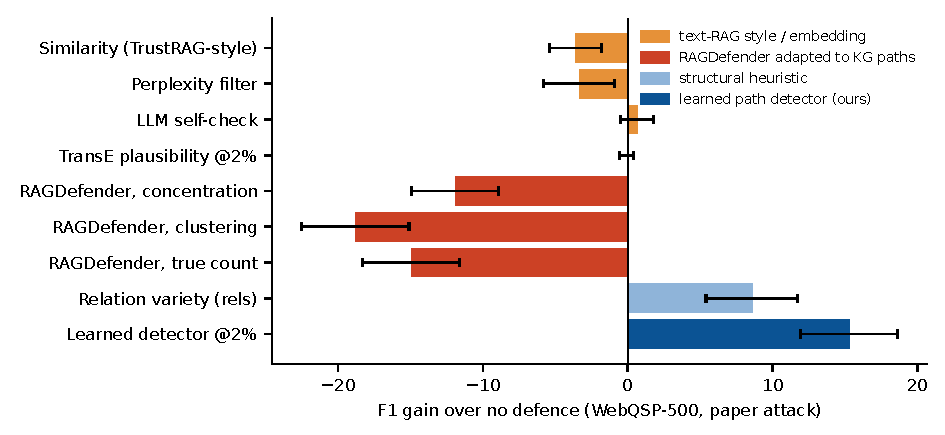
\includegraphics[width=\textwidth]{figures/fig_baselines.pdf}
\caption{F1 gain over no defence for the baselines and the learned detector (WebQSP-500, paper attack; 95\% paired bootstrap intervals). Text-RAG-style filters and the RAGDefender adaptation lower F1; only the structural heuristic and the learned detector help.}
\label{fig:baselines}
\end{figure}

\subsection{Adaptive and evasive attackers}\label{sec:adaptive}
\begin{table}[tbp]
\centering\small
\resizebox{\ifdim\width>\textwidth\textwidth\else\width\fi}{!}{%
\begin{tabular}{@{}llrr@{}}
\toprule
Attacker & Detector trained on & F1 @2\% & Gain vs none \\
\midrule
Adaptive (decoys), 500 q & paper attack only & 54.9 & $+$9.3 [$+$6.0, $+$12.4] \\
Adaptive, 500 q & paper + K1 + K8 + adaptive & 62.0 & $+$16.4 [$+$13.2, $+$19.8] \\
Adaptive, 1{,}328 q & paper attack only & 55.1 & $+$10.0 [$+$8.0, $+$11.9] \\
Adaptive, 1{,}328 q & paper + K1 + K8 + adaptive & 60.7 & $+$15.6 [$+$13.7, $+$17.6] \\
Evasive, 500 q & paper attack only & 50.1 & \textbf{$-$1.4 [$-$4.6, $+$1.9]} \\
Evasive, 500 q & paper + K1 + K8 + adaptive & 55.4 & $+$3.9 [$+$0.9, $+$6.8] \\
Evasive, 500 q & $+$ evasive (attack-aware) & 60.0 & $+$8.5 [$+$5.4, $+$11.6] \\
\bottomrule
\end{tabular}}
\caption{Learned detector at the 2\% level against the adaptive and evasive attacks. No-defence F1 is 45.6 (adaptive) and 51.5 (evasive); original labels.}
\end{table}
\textbf{Finding.} The detector generalises to decoys, partly, and fails against an attacker who removes the repeated-chain signature on which the detector relies. Performance is bounded by the attack coverage of the calibration data. (The mixed detector's $+$3.9 on the evasive attack at 500 questions does not replicate in bf16 on 1,328 questions, Section 6.13, so we read the mixed detector as level with no defence there.) For the gate detector trained on the paper attack, the question-level attack-detection AUC (attacked against clean questions) is 0.95, 0.80 and 0.73 for the paper, adaptive and evasive attacks (original labels; strict labels: 0.95, 0.78 and 0.72, and 0.94, 0.92 and 0.80 for the mixed detector). We do not claim robustness to unseen adaptive attacks; Section~\ref{sec:heldout} evaluates three held-out families.

\paragraph{Worst case and clean cost over the attacks we built (WebQSP-500).} A security evaluation should judge a defence by the attacker's best response, not by one attack. For each system we take the attack that hurts it most. The upper block uses only choices made on development data (the conformal threshold; the gate is set to flag 5\% of clean development questions); the lower block, for comparison, uses the fixed 2\% FPR level that was chosen after inspecting part of the test data. ``Mixed'' means a detector trained on the paper, $K=1$, $K=8$ and decoy attacks; ``paper'' means the paper attack only.
\begin{table}[tbp]
\centering\footnotesize
\resizebox{\textwidth}{!}{%
\begin{tabular}{@{}lrrrrrrr@{}}
\toprule
System & Clean F1 (change) & Paper & Adaptive & Evasive & Worst-case F1 & Gain vs none & Worst planted rate \\
\midrule
No defence & 67.7 & 45.9 & 45.6 & 51.5 & 45.6 & --- & 47.7\% \\
A. Conformal always-on, paper detector & 61.6 ($-$6.1) & 60.7 & 53.4 & 48.8 & 48.8 & $+$3.2 [$-$0.2, $+$6.5] & 24.8\% \\
B. Conformal always-on, mixed detector & 62.4 ($-$5.3) & 62.8 & 62.2 & 52.4 & 52.4 & $+$6.8 [$+$3.3, $+$10.2] & 16.5\% \\
C. Gate + conformal, paper detector & 67.0 ($-$0.7) & 61.6 & 49.1 & 50.7 & 49.1 & $+$3.5 [$+$1.9, $+$5.3] & 37.2\% \\
\textbf{D. Gate + conformal, mixed detector} & \textbf{67.2 ($-$0.5)} & 60.8 & 61.8 & 50.8 & 50.8 & \textbf{$+$5.2 [$+$1.9, $+$8.3]} & 25.4\% \\
\midrule
\multicolumn{8}{@{}l}{\emph{Fixed 2\% FPR level, for comparison}} \\
E. Always-on, paper detector & 61.7 ($-$5.9) & 61.1 & 54.9 & 50.1 & 50.1 & $+$4.5 [$+$1.3, $+$7.7] & 16.7\% \\
F. Always-on, mixed detector & 61.6 ($-$6.1) & 63.0 & 62.0 & 55.4 & 55.4 & $+$9.8 [$+$6.3, $+$13.3] & 11.4\% \\
G. Gate, paper detector & 67.5 ($-$0.1) & 60.8 & 48.8 & 52.4 & 48.8 & $+$3.2 [$+$1.4, $+$5.1] & 34.7\% \\
H. Gate, mixed detector & 66.9 ($-$0.7) & 62.1 & 61.8 & 51.7 & 51.7 & $+$6.1 [$+$2.9, $+$9.2] & 24.3\% \\
\bottomrule
\end{tabular}}
\caption{Clean cost and worst case over the paper, adaptive and evasive attacks. Rows C and D use strict labels; A, B and E--H keep the original labelling. Paired bootstrap intervals over questions, minimum over attacks taken inside each resample.}
\end{table}
The always-on filter has the best worst case but costs 5--6 F1 on clean graphs (Figure~\ref{fig:tradeoff}a); the gate gives up about 1.6 points of worst-case F1 to recover about five clean points, so \textbf{D is our recommended configuration}: a clean cost of $-$0.5 [$-$1.5, $+$0.4] and a worst-case gain of $+$5.2 [$+$1.9, $+$8.3]. Training on more attacks helps on the attacks it covers (Figure~\ref{fig:tradeoff}b; adaptive: 61.8 against 49.1), but the worst-case gain is not significantly larger (D against C: $+$1.7 [$-$1.3, $+$4.3] over the three known attacks; Section~\ref{sec:heldout} finds none on unseen families). Row A's worst-case gain ($+$3.2 [$-$0.2, $+$6.5]) is not significantly different from zero. \textbf{Caveats:} the worst case is over the attacks we built, not over all possible attackers; the mixed detector was trained on $K=1$ and decoy attacks and the evasive attack is $K=1$ plus decoys, so its evasive result tests a new combination of seen components, not an unseen attack family (Section~\ref{sec:heldout} tests unseen families); and on the evasive attack D is level with no defence (50.8 against 51.5): the filter lowers the planted-answer rate (from 34.5\% undefended to 25.4\% with D) but does not raise F1, because it also removes correct evidence.

\begin{figure}[tbp]
\centering
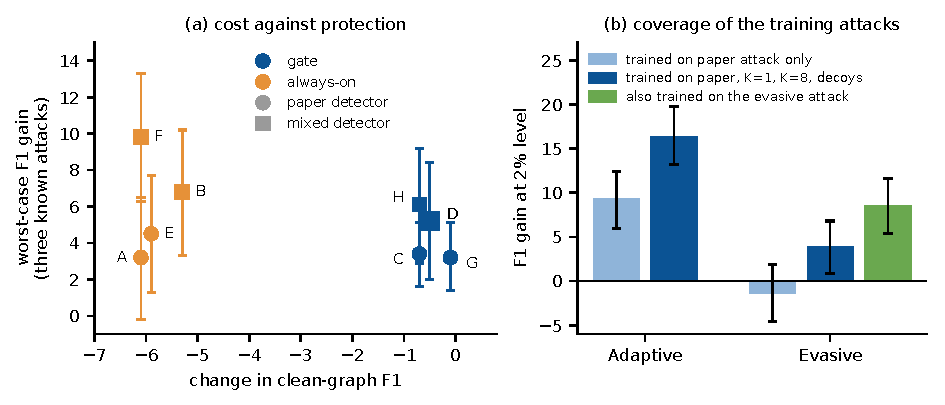
\includegraphics[width=\textwidth]{figures/fig_tradeoff_coverage.pdf}
\caption{(a) Clean-graph cost against worst-case gain over the three known attacks for configurations A--H of Section~\ref{sec:adaptive} (bars: 95\% intervals). The gate (blue) removes the clean cost of always-on filtering (orange) for a small loss of worst-case gain; D is the recommended configuration. (b) Gain at the 2\% level by what the detector was trained on: coverage of the attack matters.}
\label{fig:tradeoff}
\end{figure}

\subsection{Cost on clean graphs and the gate}\label{sec:clean}
\begin{table}[tbp]
\centering\small
\resizebox{\ifdim\width>\textwidth\textwidth\else\width\fi}{!}{%
\begin{tabular}{@{}lrr@{}}
\toprule
Defence (WebQSP-500, no attack) & F1 & Change \\
\midrule
None & 67.7 & --- \\
Learned @2\% & 61.7 & $-$5.9 [$-$8.3, $-$3.8] \\
Conformal $\alpha{=}0.05$ & 61.6 & $-$6.1 [$-$8.2, $-$3.9] \\
Learned @10\% & 42.1 & $-$25.5 [$-$29.2, $-$21.8] \\
Question-level gate, 2\% path level (5\% of clean questions) & 67.5 & $-$0.1 [$-$1.1, $+$0.7] \\
Question-level gate, conformal path level, paper detector (C) & 67.0 & $-$0.7 [$-$1.6, $+$0.2] \\
Question-level gate, conformal path level, mixed detector (D) & 67.2 & $-$0.5 [$-$1.5, $+$0.4] \\
\bottomrule
\end{tabular}}
\caption{Cost of filtering on clean graphs (WebQSP-500, no attack). Gate rows C and D use strict labels, the others the original labels.}
\end{table}
Always-on filtering costs about six F1 points on clean graphs. Runtime is not a concern: scoring the paths of a question with the detector takes about 0.1~ms on a CPU (500 questions in 0.07~s), against about one second per question for the 4-bit reasoner; the graph features (degrees, shared neighbours) are computed during retrieval and were not timed separately. The question-level gate (Section~\ref{sec:method}; \texttt{kgrag/gate.py}, flagging 5\% of clean development questions) removes that cost and keeps nearly all of the gain under the paper attack:
\begin{table}[tbp]
\centering\small
\resizebox{\textwidth}{!}{%
\begin{tabular}{@{}lrrrr@{}}
\toprule
Setting (WebQSP-500, F1) & No defence & A. Conformal always-on & C. Gate, paper det. & D. Gate, mixed det. \\
\midrule
Paper attack & 45.9 & 60.7 & 61.6 & 60.8 \\
Adaptive attack & 45.6 & 53.4 & 49.1 & 61.8 \\
Evasive attack & 51.5 & 48.8 & 50.7 & 50.8 \\
No attack & 67.7 & 61.6 & 67.0 & 67.2 \\
\bottomrule
\end{tabular}}
\caption{F1 of the dev-only variants (conformal threshold): always-on filter (A) and gate (C, D; strict labels).}
\end{table}
On clean graphs the gate costs $-$0.7 [$-$1.6, $+$0.2] F1 with the paper-attack detector (C) and $-$0.5 [$-$1.5, $+$0.4] with the mixed detector (D), against $-$6.1 for the always-on conformal filter (A). The price is coverage of unseen attacks: with a paper-attack detector the gate gives 49.1 on the adaptive attack where the always-on filter gives 53.4, because a gate trained on the paper attack flags fewer of those questions; on the evasive attack C and D are level with no defence (50.7 and 50.8 against 51.5), while A falls below it (48.8). The recommended configuration is D, the gate with the conformal threshold and the mixed-trained detector (Section~\ref{sec:adaptive}).

\subsection{Robustness checks}
\emph{Attack seeds} (new wrong answers and bridge sampling, detector fixed; WebQSP-500, learned detector trained on the paper attack, 2\% level, original labels, seed 0 being the main run): gains $+$15.3, $+$15.8, $+$14.4, $+$16.1, $+$15.6 for seeds 0--4, mean $+$15.4, s.d.\ 0.7. \emph{Second reasoner:} with Qwen2.5-7B-Instruct reading RoG's paths the gain is $+$11.2 [$+$7.9, $+$14.4] (paper attack) and $+$9.4 [$+$6.2, $+$12.7] (adaptive, attack-mixed detector). The absolute gain is smaller because that reasoner is less hurt by planted paths (planted answers 32.0\% versus 47.7\%).

\subsection{Calibration}\label{sec:calib}
In a validity simulation we pooled 800 labelled questions (the 300 development questions and the first 500 test questions, used only for this simulation and for no other reported result) and drew 100 random splits of 150 training, 250 calibration and 400 test questions (larger than the 100/200 split of the main pipeline); the realised risk is 0.045 at $\alpha=0.05$ and 0.096 at $\alpha=0.10$ (strict labels; Figure~\ref{fig:calib}): the guarantee holds on average, but individual splits can exceed $\alpha$ because it is an expectation, not a per-split bound: the realised risk is at most $\alpha$ in 63\% of splits at $\alpha=0.05$, 55\% at $\alpha=0.10$, 66\% at $\alpha=0.02$ and 58\% at $\alpha=0.20$. On single test splits at $\alpha=0.05$ the realised risk is 0.048--0.058 on the attack used for calibration, 0.060--0.104 on the adaptive attack and the three held-out families, and 0.16--0.18 on the unseen evasive attack (mixed and paper detector respectively), so calibration on one attack does not protect against another. On the full test sets the realised risk of the conformal threshold calibrated on the paper attack is 0.077 (WebQSP-1328) and 0.071 (CWQ-3231), above the target. The mixed detector is calibrated on four attack versions of the same development questions (about 680 rows from about 170 distinct answerable questions), so the sample size n in the bound counts correlated rows and overstates the number of independent questions. Calibrating on a mix of the paper and adaptive attacks restores the level for both (0.053 and 0.050 in the simulation) but not for an attack outside the mix. On the full set the calibrated threshold gives $+$14.9 [$+$12.8, $+$17.0] (WebQSP) and $+$7.9 [$+$6.5, $+$9.3] (CWQ), with strict labels (Section~\ref{sec:main}).

\begin{figure}[tbp]
\centering
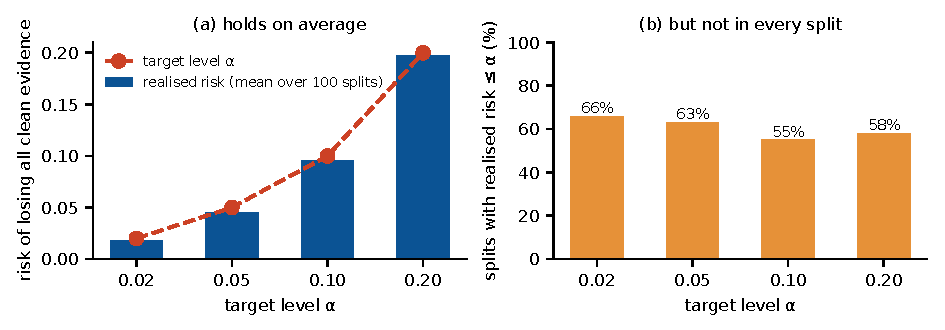
\includegraphics[width=\textwidth]{figures/fig_calibration.pdf}
\caption{Conformal validity in the 100-split simulation of Section~\ref{sec:calib}. (a) The mean realised risk matches the target level. (b) It is an expectation: only 55--66\% of individual splits stay within the target.}
\label{fig:calib}
\end{figure}

\subsection{GCR: the attack and the defence on a second system}\label{sec:gcr}
Our GCR pipeline follows the original: the fine-tuned GCR model generates constrained reasoning paths (10 beams; plain beam search because group beam search needs \texttt{trust\_remote\_code}; 4-bit), then a general LLM reads the paths and answers. We use Qwen2.5-7B-Instruct as that reasoner, where Zhao et al.\ use GPT-3.5-turbo.
\begin{table}[tbp]
\centering\small
\resizebox{\textwidth}{!}{%
\begin{tabular}{@{}lrrrrr@{}}
\toprule
WebQSP, 400 q & Hit & F1 & Hits@1 & EM & Planted top-1 \\
\midrule
Clean & 82.0 & 65.2 & 71.2 & 39.2 & --- \\
Attacked & 81.2 & 60.7 & 68.0 & 29.2 & 3.2\% \\
Change & $-$0.8 [$-$2.0, $+$0.2] & $-$4.5 [$-$6.2, $-$3.0] ($-$7\%) & $-$3.2 [$-$5.0, $-$1.8] ($-$5\%) & $-$10.0 [$-$13.0, $-$7.2] ($-$25\%) & \\
\bottomrule
\end{tabular}}
\caption{GCR with a second-stage reasoner, clean versus attacked graph (pilot on the first 400 WebQSP test questions, 4-bit, paper attack).}
\end{table}
The 400-question table is a pilot on test questions 0 to 399, run before the defence work; the defence experiments below need the beam paths of every question, so they come from a separate pass over the 1{,}328 attacked and 500 clean questions, which is why the clean F1 differs (65.2 on 400 questions, 63.8 on 500). Zhao et al.\ report for GCR with a GPT-3.5-turbo reasoner: clean F1 71.07, Hits@1 78.50, EM 44.29, and attacked drops of F1 $-$10\%, Hits@1 $-$12\%, EM $-$22\%. Our clean numbers are lower (a different reasoner), but the effect sizes are comparable (EM $-$25\% against $-$22\%, F1 $-$7\% against $-$10\%). The attack therefore \textbf{does} reduce GCR's accuracy, moderately and less than RoG's. The first stage alone is barely affected (F1 35.7 to 34.9, planted answer on top in 2.5\% of questions; 3.0\% under the stronger $N=10$, $K=8$ budget): the damage happens in the second stage, where planted paths that survive the trie mislead the reasoner. \paragraph{The defence on GCR.} We put the same filter between GCR's first stage and its second-stage reasoner (\texttt{kgrag/gcr\_defend.py}). The unique beam paths of each question (about 7.3 per question) are turned into the per-path records used for RoG, with strict labels; 5.1\% of beam paths are poisoned and 198 of the 1,328 attacked test questions (15\%) have at least one. Variants: \emph{transfer} = the RoG-trained mixed detector with the conformal threshold recalibrated on GCR development beams; \emph{fitted} = a detector trained on the first 100 GCR development questions and calibrated on the other 200; \emph{D} = the recommended gate (RoG-trained detector, threshold recalibrated on 300 clean GCR development questions) in front of the transferred conformal filter; \emph{oracle} removes the poisoned beam paths. The test set is the 1,328 WebQSP questions, 500 clean questions measure the cost, and every variant covers exactly the same questions.
\begin{table}[tbp]
\centering\footnotesize
\resizebox{\textwidth}{!}{%
\begin{tabular}{@{}lrrrrr@{}}
\toprule
GCR, WebQSP-1328 (clean: 500 q) & None & Oracle & Transfer & Fitted & D (gate) \\
\midrule
F1, attacked & 58.0 & 60.2 ($+$2.2 [$+$1.5, $+$3.0]) & 53.4 ($-$4.6 [$-$5.9, $-$3.5]) & 57.2 ($-$0.8 [$-$1.8, $+$0.1]) & 57.2 ($-$0.8 [$-$1.4, $-$0.1]) \\
EM, attacked & 28.2 & 33.5 ($+$5.3 [$+$4.1, $+$6.6]) & 25.6 ($-$2.6 [$-$4.1, $-$1.1]) & 27.0 ($-$1.1 [$-$2.6, $+$0.3]) & 28.4 ($+$0.2 [$-$0.5, $+$1.0]) \\
Hits@1, attacked & 63.7 & 64.2 & 60.2 & 62.5 & 63.0 \\
Planted answer top-1 & 4.7\% & 3.1\% & 4.4\% & 3.9\% & 4.4\% \\
Beam paths kept & 100\% & 95\% & 82\% & 92\% & 96\% \\
F1, questions with a poisoned beam path (198) & --- & $+$15.0 [$+$10.2, $+$19.6] & $-$0.8 [$-$5.3, $+$3.5] & $+$7.2 [$+$2.9, $+$11.5] & $+$2.0 [$-$0.9, $+$5.0] \\
F1, clean graph (500 q) & 63.8 & --- & 58.8 ($-$5.0 [$-$6.7, $-$3.3]) & 61.4 ($-$2.4 [$-$3.6, $-$1.3]) & 62.8 ($-$1.0 [$-$1.8, $-$0.4]) \\
\bottomrule
\end{tabular}}
\caption{The defence on GCR (strict labels; paired differences against no defence in parentheses).}
\end{table}
\textbf{Finding: on GCR the defence does not pay} (Figure~\ref{fig:gcr}). The headroom is small, $+$2.2 F1 for a perfect filter, because the second-stage reasoner puts a planted answer first in only 4.7\% of questions. The detector does find poisoned beam paths (path-level AUC 0.77 for the RoG-trained mixed detector on GCR beams, against 0.96 on RoG's own paths; strict labels), and the fitted detector gains $+$7.2 [$+$2.9, $+$11.5] on the 15\% of questions that have one, but it also removes correct beam paths in the other 85\%, and the net effect is $-$0.8 [$-$1.8, $+$0.1] on attacked data and $-$2.4 [$-$3.6, $-$1.3] on clean data. The gate recovers most of the clean cost ($-$1.0 against $-$2.4 and $-$5.0) and is level with no defence on exact match ($+$0.2 [$-$0.5, $+$1.0]) but not better. The questions with a poisoned beam path were designated as a secondary analysis in the code before the final strict-label runs (git history, 9 October 2026). \textbf{Where the damage goes (500 questions).} The clean run covers the first 500 questions, which are also attacked, so the damage can be decomposed on those (the other 828 attacked questions have no clean run). There the attack costs 4.8 F1 [3.3, 6.3] (clean 63.8, attacked 59.0). Removing exactly the poisoned paths (the oracle) gives back 2.4 [1.1, 3.8]; the other 2.4 [1.3, 3.7] stays lost. More than nine tenths of that remainder sits in the 9\% of questions (47 of 500) in which a clean gold-supporting beam path is missing from the attacked run's non-poisoned paths: there the oracle leaves a loss of 23.7 F1 [14.4, 33.9], against 0.2 [$-$0.3, $+$0.8] in the other 453 questions. Of the 65 missing paths, 61 (94\%) run through an entity pair that carries an inserted triple with a different relation. GCR builds its graph with one relation per directed entity pair (\texttt{build\_graph} in its repository, \texttt{nx.DiGraph.add\_edge}), so such a triple replaces the clean relation, the same overwriting that separates the oracle from the clean graph for RoG (Section 6.12). Half of GCR's damage is therefore clean evidence that has been replaced, and no filter applied to the remaining paths can bring it back. Among the 74 questions with a poisoned beam path the oracle recovers 16.3 of a 23.4 F1 loss; among the 426 without one it recovers nothing, and the 1.6 F1 lost there is replaced evidence.

\begin{figure}[tbp]
\centering
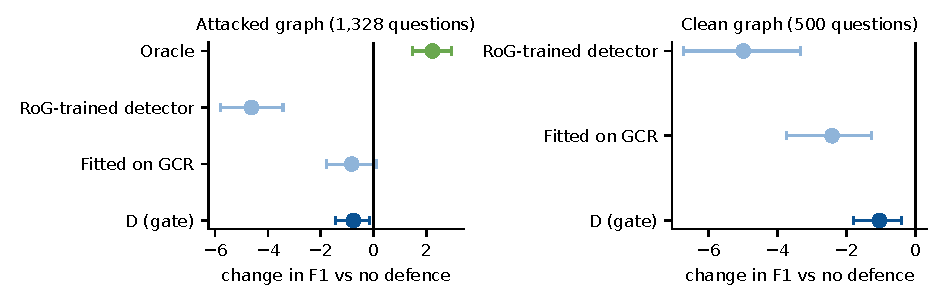
\includegraphics[width=\textwidth]{figures/fig_gcr.pdf}
\caption{GCR: change in F1 against no defence, with 95\% paired bootstrap intervals. A perfect filter (oracle) gains only 2.2 points on the attacked graph; none of the detectors improves on no defence, and all of them cost accuracy on the clean graph.}
\label{fig:gcr}
\end{figure}

\subsection{Stronger attack budget}\label{sec:budget}
Ten wrong answers and up to eight triples each, with the detector trained on the paper attack only.
\begin{table}[tbp]
\centering\small
\resizebox{\ifdim\width>\textwidth\textwidth\else\width\fi}{!}{%
\begin{tabular}{@{}lrrrr@{}}
\toprule
Defence & F1 & Hit & Planted answer & F1 gain vs none \\
\midrule
None & 42.1 [38.7, 45.4] & 75.0 [71.2, 78.8] & 48.6\% & --- \\
Learned @2\% & 57.9 [54.8, 61.1] & 80.2 & 23.4\% & $+$15.9 [$+$13.0, $+$19.0] \\
Conformal $\alpha{=}0.05$ & 60.0 [56.5, 63.2] & 80.2 & 17.2\% & $+$17.9 [$+$14.7, $+$21.2] \\
Oracle & 64.4 [61.0, 67.8] & 81.2 & 3.0\% & $+$22.4 [$+$18.9, $+$26.0] \\
\bottomrule
\end{tabular}}
\caption{Stronger attack budget ($N=10$, $K=8$), WebQSP-500, original labels (including the oracle), detector trained on the paper attack only.}
\end{table}
The oracle row keeps the original labels (there is no strict run for this budget). The equal Hit of 80.2 for the learned and conformal rows is a coincidence: 401 of 500 questions each, with 32 questions differing. The larger budget does more damage (F1 $-$38\% and Hit $-$10\% relative to the clean graph, against $-$32\% and $-$6\% for the paper attack). The unseen detector still recovers 80.0\% [69.9, 90.7] of the oracle gain with the conformal threshold and 70.9\% [60.4, 82.6] with the fixed 2\% level; the conformal threshold does better here because it removes more paths (42\% kept, against 54\%) when the attack inserts more.

\subsection{Held-out attack families}\label{sec:heldout}
The detector, the conformal threshold and the gate are fitted on the paper, $K=1$, $K=8$ and decoy attacks (``mixed'') or on the paper attack alone, and tested on three families built after the detector was fixed (descriptions in Section~\ref{sec:threat}). None uses the gold answers.
\begin{table}[tbp]
\centering\footnotesize
\resizebox{\textwidth}{!}{%
\begin{tabular}{@{}lrrrr@{}}
\toprule
System & Profile-copy & Bridge & Spread & Worst case \\
\midrule
No defence & 45.8 & 43.5 & 43.4 & 43.4 \\
Oracle (strict) & 65.4 & 66.0 & 65.7 & 65.4 \\
Conformal always-on, mixed & 54.6 ($+$8.8 [$+$6.0, $+$11.7]) & 56.4 ($+$12.9 [$+$9.6, $+$15.9]) & 59.2 ($+$15.8 [$+$12.8, $+$18.8]) & 54.6 ($+$11.3 [$+$8.2, $+$13.6]) \\
\textbf{Gate + conformal, mixed} & 52.3 ($+$6.5 [$+$4.0, $+$8.9]) & 56.1 ($+$12.6 [$+$9.8, $+$15.4]) & 57.6 ($+$14.2 [$+$11.2, $+$17.3]) & \textbf{52.3 ($+$8.9 [$+$5.7, $+$11.2])} \\
Gate + conformal, paper detector & 52.9 ($+$7.1 [$+$4.9, $+$9.4]) & 56.3 ($+$12.8 [$+$9.7, $+$15.9]) & 57.6 ($+$14.2 [$+$11.1, $+$17.4]) & 52.9 ($+$9.5 [$+$6.5, $+$11.7]) \\
\bottomrule
\end{tabular}}
\caption{F1 on three held-out attack families (oracle and gate rows use strict labels; the always-on row keeps the original labelling), with the paired gain over no defence in brackets; paired bootstrap over questions, minimum over families inside each resample.}
\end{table}
\textbf{Findings.} (i) The gains are positive and clearly above zero on all three families: the recommended gate recovers 33\% (profile-copy), 56\% (bridge) and 64\% (spread) of the oracle gain, against 76\% (paper) and 82\% (adaptive) on the attacks used for training; the profile-copy attack, which copies the profile of a real endpoint, is the hardest. Shares are taken against the strict oracle of each attack on WebQSP-500: 65.4 (paper), 65.4 (adaptive), 66.4 (evasive), 65.4 (profile-copy), 66.0 (bridge) and 65.7 (spread). (ii) The conformal always-on filter (original labels, divided by the strict-oracle gain) recovers more (45\%, 57\%, 71\%) at the clean-data cost of Section~\ref{sec:adaptive}. (iii) Training on more attacks does not help beyond the attacks it covers: the paper-only detector reaches the same worst case (D minus C: $-$0.6 [$-$2.4, $+$1.2]), so the benefit of mixed training seen on the adaptive attack (61.8 against 49.1, Section~\ref{sec:adaptive}) does not carry over to these families. (iv) The mixed detector's path-level AUC is 0.89 (profile-copy), 0.88 (bridge) and 0.94 (spread), against 0.95 on the paper attack. \textbf{Caveat:} the families are our own constructions, built after we knew which features the detector uses and not optimised against the final detector; a stronger adaptive attacker may do better.

\paragraph{Worst case over all six attacks (WebQSP-500; $n=500$, the same questions for every attack).} The held-out families do more damage undefended (worst case 43.4, against 45.6 on the known attacks), so the gains quoted separately for the known attacks ($+$5.2, Section~\ref{sec:adaptive}) and for the held-out families ($+$8.9) are not comparable; the single worst case over all six is the fair headline (Figure~\ref{fig:six}).
\begin{table}[tbp]
\centering\footnotesize
\resizebox{\textwidth}{!}{%
\begin{tabular}{@{}lrrrrrrrrr@{}}
\toprule
System & Paper & Adapt. & Evasive & Profile & Bridge & Spread & Worst-case F1 & Gain vs none & Worst planted \\
\midrule
No defence & 45.9 & 45.6 & 51.5 & 45.8 & 43.5 & 43.4 & 43.4 (spread) & --- & 50.7\% \\
B. Conformal always-on, mixed & 62.8 & 62.2 & 52.4 & 54.6 & 56.4 & 59.2 & 52.4 (evasive) & $+$9.0 [$+$5.7, $+$11.8] & 22.7\% \\
C. Gate + conformal, paper det. & 61.6 & 49.1 & 50.7 & 52.9 & 56.3 & 57.6 & 49.1 (adaptive) & $+$5.7 [$+$3.3, $+$7.5] & 37.2\% \\
\textbf{D. Gate + conformal, mixed} & 60.8 & 61.8 & 50.8 & 52.3 & 56.1 & 57.6 & 50.8 (evasive) & \textbf{$+$7.4 [$+$4.5, $+$9.9]} & 29.8\% \\
\bottomrule
\end{tabular}}
\caption{F1 under six attacks and the worst case over them; rows C and D use strict labels, row B keeps the original labelling; paired bootstrap intervals, minimum over attacks inside each resample.}
\end{table}
Row A (the paper-detector always-on filter) was not run on the held-out families. \textbf{Coverage helps on the attacks it covers, not beyond them:} the mixed detector D beats the paper-only detector C on the adaptive attack (61.8 against 49.1), but the worst-case difference D minus C is $+$1.7 [$-$1.3, $+$4.3] over the three known attacks and $-$0.6 [$-$2.4, $+$1.2] on the held-out families, so neither is distinguishable from zero. On the evasive attack D is level with no defence (50.8 against 51.5).

\begin{figure}[tbp]
\centering
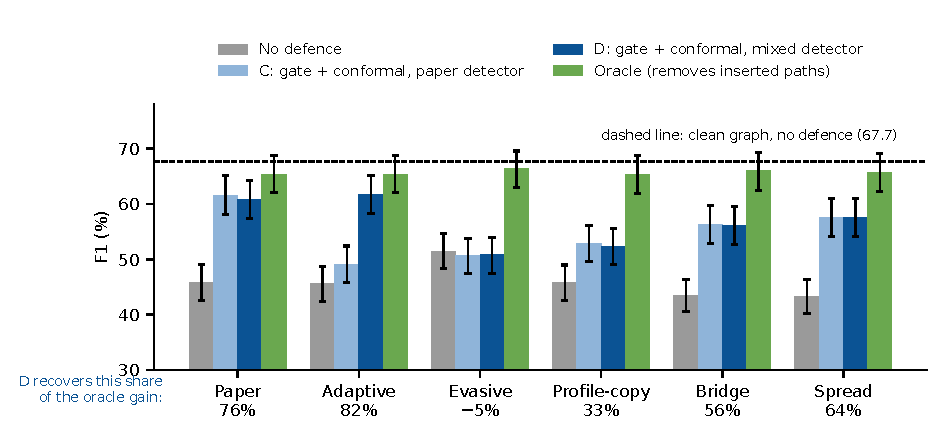
\includegraphics[width=\textwidth]{figures/fig_six_attacks.pdf}
\caption{F1 on WebQSP-500 under the six attacks, with 95\% bootstrap intervals over questions. Under each attack name: the share of the oracle gain recovered by D. Rows C, D and the oracle use strict labels. D is level with no defence on the evasive attack and recovers 33\% on the hardest held-out family.}
\label{fig:six}
\end{figure}

\subsection{The gate on CWQ and a KG-embedding feature}\label{sec:cwqkge}
\emph{CWQ} (3{,}231 questions; detector fitted on WebQSP development data only): the gate with the conformal threshold (detector C, trained on the paper attack) gains $+$7.7 [$+$6.4, $+$9.1] F1 (conformal always-on $+$8.0 [$+$6.6, $+$9.4]; oracle $+$11.4 [$+$9.8, $+$13.0]; these CWQ gate rows keep the original labelling, under which the oracle gain is $+$11.4, against $+$13.1 [$+$11.7, $+$14.6] with strict labels) and leaves 17.7\% planted answers (the gate flags 9.3\% of the clean CWQ questions that have a retrieved path, against its 5\% target on WebQSP development questions, and 82\% of the attacked ones); on the clean CWQ graph it costs $-$1.3 [$-$1.8, $-$0.8] F1 (48.8 to 47.5; 48.8 is the clean run through the same path pipeline, 48.9 the end-to-end clean run of Section~\ref{sec:main}). \emph{TransE as a detector feature} (four extra features: minimum and mean path plausibility, share of unscored triples, per-question z-score of the minimum), WebQSP-500 attacks, original labels; paired F1 difference as with the feature minus without it, gate + conformal, mixed detector: paper $+$0.4 [$-$1.3, $+$2.1], evasive $+$0.1 [$-$2.2, $+$2.2], profile-copy $+$1.8 [$+$0.2, $+$3.4], bridge $+$4.0 [$+$2.2, $+$5.9], spread $+$0.9 [$-$0.9, $+$2.7], clean $-$0.1 [$-$0.9, $+$0.7]. It helps on the unseen bridge attack (conformal always-on: $+$3.1 [$+$1.4, $+$4.9]) and slightly on profile-copy, but not on the evasive attack, so it does not close the evasive gap.

\subsection{Does the oracle gap come from RoG's graph representation?}\label{sec:multigraph}
RoG builds a networkx Graph with one relation per entity pair, so an inserted triple on an existing pair overwrites the clean relation. We repeat the paper attack (WebQSP-500) with retrieval on a MultiGraph that keeps every parallel edge (path features still use the simple graph; strict labels; the mixed detector, the conformal threshold and the gate are rebuilt on MultiGraph development paths, 66 paths per question against 36).
\begin{table}[tbp]
\centering\small
\begin{tabular}{@{}lrrrrr@{}}
\toprule
Retrieval graph & Clean & No defence & Oracle & D & D on clean \\
\midrule
Simple graph (RoG) & 67.7 & 45.9 & 65.4 & 60.8 & 67.2 \\
MultiGraph & 74.6 & 42.0 & 74.6 & 66.1 & 74.4 \\
\bottomrule
\end{tabular}
\caption{MultiGraph ablation, WebQSP-500, paper attack, strict labels, F1.}
\end{table}
On the MultiGraph the oracle returns exactly to the clean level (74.6 against 74.6; Figure~\ref{fig:mg}), and the retained path set is identical to the clean one in all 500 questions, which holds by construction because retrieval has no path cap and no clean edge is overwritten. This shows that overwriting by the simple graph accounts for the whole gap between the oracle and the clean graph in the main experiments (65.4 against 67.7), not label noise; it is a consistency check of the oracle and the labels rather than an independent measurement. The simple graph also loses clean evidence without any attack (clean F1 67.7 against 74.6): the main experiments follow RoG's released graph construction, and a reader may ask why they do not use the stronger retrieval. The attack is also stronger when parallel edges survive: $-$32.6 F1 against $-$21.8 on the simple graph. D recovers $+$24.0 [$+$20.9, $+$27.2] of an oracle gain of $+$32.6 [$+$29.5, $+$35.8], about 74\%, at a clean cost of $-$0.2 [$-$0.9, $+$0.5]. The main-body numbers therefore understate the attack on a graph store that keeps parallel edges, and the defence keeps about the same share of the oracle gain. With parallel edges kept, Hit rises from 83.2 to 88.6, precision from 77.0 to 80.9 and recall from 72.8 to 80.0 on the clean graph, so the gain is not more answers at lower precision. This was measured on the 500-question subset only, with our own 4-bit retrieval implementation, so we make no comparison with published RoG numbers.

\begin{figure}[tbp]
\centering
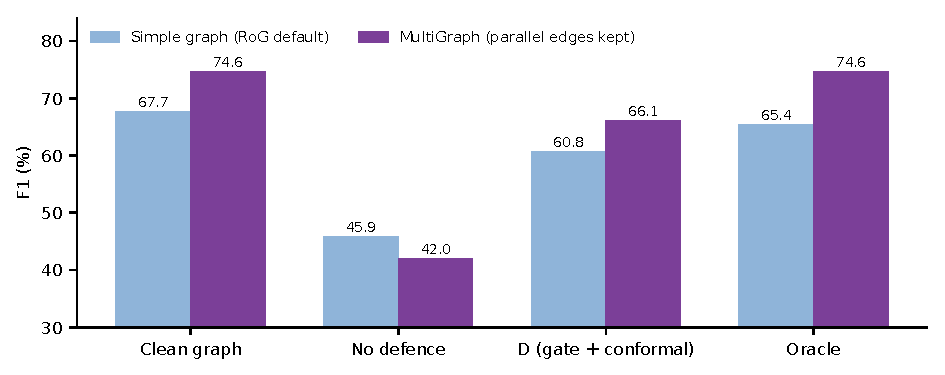
\includegraphics[width=\textwidth]{figures/fig_multigraph.pdf}
\caption{MultiGraph ablation (WebQSP-500, paper attack, strict labels). Keeping parallel edges closes the gap between the oracle and the clean graph (74.6 against 74.6), makes the attack stronger, and D recovers about three quarters of the oracle gain.}
\label{fig:mg}
\end{figure}

\subsection{Full-precision (bf16) check}\label{sec:bf16}
The same defences were rerun on a compute cluster with bf16 weights (WebQSP-1328; detectors and thresholds unchanged). Paired differences, bf16 minus the 4-bit run:
\begin{table}[tbp]
\centering\small
\begin{tabular}{@{}lrrr@{}}
\toprule
Setting (WebQSP-1328) & 4-bit & bf16 & Difference \\
\midrule
Paper, no defence & 45.3 & 46.1 & $+$0.8 [$-$0.1, $+$1.7] \\
Paper, oracle & 65.5 & 66.3 & $+$0.8 [0.0, $+$1.6] \\
Paper, conformal $\alpha$=0.05 & 60.3 & 60.8 & $+$0.5 [$-$0.2, $+$1.3] \\
Paper, learned @2\% & 61.2 & 62.1 & $+$0.9 [$+$0.1, $+$1.8] \\
Paper, rels & 54.4 & 55.4 & $+$1.0 [$+$0.2, $+$1.9] \\
Adaptive, no defence & 45.1 & 46.2 & $+$1.1 [$+$0.2, $+$2.0] \\
Adaptive, oracle & 65.6 & 66.3 & $+$0.7 [$-$0.1, $+$1.5] \\
Adaptive, learned (mixed) @2\% & 60.7 & 60.8 & $+$0.2 [$-$0.8, $+$1.1] \\
Adaptive, learned (paper) @2\% & 55.1 & 55.9 & $+$0.8 [$-$0.2, $+$1.8] \\
\bottomrule
\end{tabular}
\caption{Full precision (bf16) against the 4-bit run, WebQSP-1328, F1, original labels for every row; paired differences.}
\end{table}
Full precision raises every row by 0.2 to 1.1 F1 (about 0.8 on average), no-defence and defended alike, so the gains do not change (conformal threshold, original labels: $+$14.7 in bf16, $+$15.0 in 4-bit). The evasive attack on all 1,328 questions (K=1 plus 12 decoys) gives no defence 51.2, oracle 66.5, a detector trained on the paper attack only 49.0, the mixed detector 51.1 and the attack-aware detector 58.4; the conformal rows give 50.4 (mixed) and 58.2 (attack-aware). The mixed detector therefore gains nothing on the evasive attack at this size ($-$0.1), whereas the 500-question 4-bit run gave $+$3.9 [$+$0.9, $+$6.8] (Section 6.4). On the same first 500 questions the bf16 run gives $+$1.9 [$-$1.4, $+$5.0] (no defence 51.8, mixed detector 53.7), and on the other 828 questions $-$1.2 [$-$3.8, $+$1.4]: about half of the 4-bit gain disappears at full precision on identical questions, and the remaining questions do not show it. We did not rerun this attack in 4-bit on all 1,328 questions: the 500-question 4-bit rows and the 1,328-question bf16 rows agree that the mixed detectors are level with no defence on the evasive attack, so we do not claim the $+$3.9 as a gain. All rows of this table, including the oracle and conformal rows, use the original labelling, so its 4-bit column is the original-label run (oracle 65.5 and conformal 60.3 here, against 65.6 and 60.1 with strict labels in Section 6.2; the conformal gain is $+$15.0 here and $+$14.9 with strict labels). The strict reruns are 4-bit only.

\section{Limitations}
\begin{itemize}[leftmargin=*,itemsep=2pt]
\item \textbf{Attack strength.} Our reproduced attack is weaker than the original at the paper settings; the larger budget of Section~\ref{sec:budget} narrows the gap on Hit but not on EM ($-$58\% against $-$81\%) (Sections~\ref{sec:attack}, \ref{sec:budget}).
\item \textbf{Unseen adaptive attackers.} The defence needs attack coverage in the calibration data; an evasive attacker defeats an unseen detector (Section~\ref{sec:adaptive}).
\item \textbf{Held-out families are our own.} The three held-out families (Section~\ref{sec:heldout}) were built after we knew which features the detector uses and were not optimised against the final detector; on them the gain is 33--64\% of a perfect filter's, and mixed training does not help beyond the paper-only detector. The mixed detector's evasive result (Section~\ref{sec:adaptive}) combines seen components.
\item \textbf{Clean-data cost.} The always-on filter costs about 6 F1 on clean graphs; the gate repairs this but weakens coverage of unseen attacks (Section~\ref{sec:clean}).
\item \textbf{Guarantee scope.} The conformal bound is in expectation, requires exchangeability and attack-representative calibration data, and is violated under attack shift (Section~\ref{sec:calib}).
\item \textbf{Systems.} The defence is built for RoG-style path retrieval. On GCR the attack transfers but the defence does not recover the (small) loss (Section~\ref{sec:gcr}); we have not tried SubgraphRAG or G-Retriever. Most results are 4-bit; a bf16 check on 1,328 questions agrees within 1.1 F1 (Section~\ref{sec:bf16}), but the strict-label and held-out rows are 4-bit only.
\item \textbf{Operating point.} The 2\% FPR level was fixed after inspecting part of the test data.
\item \textbf{Coverage of the recommended configuration.} D was run on WebQSP-500 (known and held-out attacks), GCR and the MultiGraph ablation, not on the 1{,}328- and 3{,}231-question sets, whose headline rows use the always-on conformal filter (A). The conformal bound is violated on those sets (realised risk 0.077 and 0.071 at a target of 0.05).
\item \textbf{Baseline operating points.} The baselines of Section~\ref{sec:baselines} are not compared at one common false-positive rate.
\item \textbf{Retrieval graph.} The main experiments use RoG's one-relation-per-pair graph; a MultiGraph store gives a stronger clean system and a stronger attack (Section~\ref{sec:multigraph}).
\item \textbf{Labelling.} Strict labels are used for C, D, the oracle, and A on WebQSP-1328 and CWQ-3231 only; other rows keep the original labelling (Section~\ref{sec:setup}).
\item \textbf{Generator.} Wrong answers come from a 7B open model, not GPT-4, and are not filtered against the gold answers (13.4\% of WebQSP-500 questions have a wrong answer that is also a gold answer, Section~\ref{sec:threat}).
\item \textbf{Datasets.} Freebase-based WebQSP and CWQ; production GraphRAG systems are not covered.
\end{itemize}

\section{Conclusion}
Poisoned KG-RAG paths are detectable from graph structure, and a calibrated filter, applied only to questions that look attacked, recovers a substantial part of the lost accuracy at almost no cost on clean graphs: about three quarters of a perfect filter's gain on the attacks it was calibrated on and a third to two thirds on attack families it never saw. Text-RAG defences and a stand-alone KG-embedding plausibility filter do not help (the embedding helps only as a detector feature, and only on one unseen attack), a defence trained on known attacks is only partly protective against new ones, and an attacker who knows the features can reduce the gain further; evaluations that omit adaptive and held-out attacks overstate robustness. The evidence is for one defended system (RoG, where bf16 reruns agree with the 4-bit numbers): on GCR the attack transfers but a perfect filter would add only $+$2.2 F1, because about half of the damage there is clean evidence overwritten by inserted triples, which no path filter can restore, and our detectors do not recover the rest; the result is a defence for settings where inserted paths are the main source of damage, not a general one.

\section*{CRediT authorship contribution statement}
\textbf{Manish Nandish:} Conceptualization, Methodology, Software, Investigation, Formal analysis, Data curation, Visualization, Writing -- original draft.
\textbf{Rajiv Misra:} Supervision, Writing -- review \& editing.
\textbf{Midhunchakkaravarthy Janarthanan:} Supervision, Writing -- review \& editing.

\section*{Declaration of competing interest}
The authors declare that they have no known competing financial interests or personal relationships that could have appeared to influence the work reported in this paper.

\section*{Funding}
This research received no funding.

\section*{Data availability}
The benchmarks (WebQSP and CWQ) and the models (RoG, GCR, Qwen2.5-7B-Instruct) are public. The attack and defence code, the poisoned-graph generators and the per-question result files will be released publicly on acceptance and are available from the corresponding author on request.

\section*{Declaration of generative AI and AI-assisted technologies in the manuscript preparation process}
During the preparation of this work the authors used Claude (Anthropic) to assist with writing and debugging code, running and checking analyses, and drafting and editing text. After using this tool, the authors reviewed and edited the content as needed and take full responsibility for the content of the published article.

\appendix
\section{Reproducibility}\label{app:repro}
\begin{sloppypar}
Code and run files are in the private repository \texttt{Manish06N/kgrag-poisoning-defence}. Tables are regenerated with \texttt{python -m kgrag.report}; the review checks with \texttt{scripts/review\_checks.py} and \texttt{scripts/gcr\_rescore.py}. Local runs used a 16~GB GPU, 4-bit nf4 weights and transformers 4.57.6. HPC (bf16) runs write to \texttt{runs/kg\_bf16/} via the environment variable \texttt{KG\_RUNS}. HPC reproduction check (job T0, 50 clean WebQSP questions): 4-bit F1 69.0, identical to the laptop run; bf16 F1 66.4 (9 of 50 predictions differ, too few to say whether this is noise); full-set (1,328 question) bf16 results are in Section~\ref{sec:bf16} (archive \texttt{results\_bf16\_T1\_2026-10-09.tar.gz}, SHA-256 prefix f0fb13733cae1b71). Strict-label reruns write to \texttt{runs/kg\_strict/} and the MultiGraph ablation to \texttt{runs/kg\_mg/} via \texttt{KG\_RUNS}; \texttt{scripts/gcr\_defence\_report.py} regenerates the GCR table and \texttt{scripts/make\_figures.py} the data figures.

\end{sloppypar}

\begin{thebibliography}{99}\small
\bibitem{zhao2025} T.~Zhao, J.~Chen, Y.~Ru, H.~Zhu, N.~Hu, J.~Liu, and Q.~Lin. Exploring knowledge poisoning attacks to retrieval-augmented generation. \emph{Information Fusion}, 127:103900, 2026, doi:10.1016/j.inffus.2025.103900 (arXiv:2507.08862, first titled ``RAG Safety: Exploring Knowledge Poisoning Attacks to Retrieval-Augmented Generation'').
\bibitem{luo2024rog} L.~Luo, Y.-F.~Li, G.~Haffari, and S.~Pan. Reasoning on Graphs: Faithful and Interpretable Large Language Model Reasoning. In \emph{ICLR}, 2024 (arXiv:2310.01061).
\bibitem{luo2024gcr} L.~Luo, Z.~Zhao, G.~Haffari, Y.-F.~Li, C.~Gong, and S.~Pan. Graph-constrained Reasoning: Faithful Reasoning on Knowledge Graphs with Large Language Models. In \emph{ICML}, 2025 (arXiv:2410.13080).
\bibitem{he2024gretriever} X.~He, Y.~Tian, Y.~Sun, N.~V. Chawla, T.~Laurent, Y.~LeCun, X.~Bresson, and B.~Hooi. G-Retriever: Retrieval-Augmented Generation for Textual Graph Understanding and Question Answering. In \emph{Advances in Neural Information Processing Systems (NeurIPS)}, vol.~37, pp.~132876--132907, 2024 (arXiv:2402.07630).
\bibitem{li2025subgraphrag} M.~Li, S.~Miao, and P.~Li. Simple Is Effective: The Roles of Graphs and Large Language Models in Knowledge-Graph-Based Retrieval-Augmented Generation. In \emph{ICLR}, 2025 (arXiv:2410.20724).
\bibitem{mavromatis2024} C.~Mavromatis and G.~Karypis. GNN-RAG: Graph Neural Retrieval for Efficient Large Language Model Reasoning on Knowledge Graphs. In \emph{Findings of the Association for Computational Linguistics: ACL 2025}, pp.~16682--16699, doi:10.18653/v1/2025.findings-acl.856 (arXiv:2405.20139, first titled ``GNN-RAG: Graph Neural Retrieval for Large Language Model Reasoning'').
\bibitem{zhou2025trustrag} H.~Zhou, K.-H. Lee, Z.~Zhan, Y.~Chen, Z.~Li, Z.~Wang, H.~Haddadi, and E.~Yilmaz. TrustRAG: Enhancing Robustness and Trustworthiness in Retrieval-Augmented Generation. arXiv:2501.00879, 2025.
\bibitem{xiao2026logic} Y.~Xiao, J.~Chen, Q.~Zhang, Y.~Zhang, C.~Zhou, L.~Yang, L.~Ren, X.~Yang, and X.~Huang. LogicPoison: Logical Attacks on Graph Retrieval-Augmented Generation. arXiv:2604.02954, 2026.
\bibitem{zheng2026trigger} Z.~Zheng, Y.-J. Choi, C.~Huang, H.~Cao, S.~Tian, and T.~Pei. Trigger as Entity: Backdoor Attacks to Graph-Based Retrieval-Augmented Generation of Large Language Models. \emph{IEEE Transactions on Information Forensics and Security}, 21:5583--5596, 2026, doi:10.1109/TIFS.2026.3699202.
\bibitem{park2026hop} J.~Park, J.~Le, and H.~Cooper. Hop-Decayed Influence: New Vulnerabilities of Structural Auxiliary Indexing in GraphRAG Pipelines with LLM. In \emph{ICT Systems Security and Privacy Protection (IFIP SEC 2026)}, IFIP AICT vol.~787, pp.~345--358, Springer, 2026 (arXiv:2610.02373).
\bibitem{kereopa2026} B.~Kereopa-Yorke, G.~Diaz, H.~Wright, R.~Johnston, R.~F. Del Rosario, and T.~Lynar. Oracle Poisoning: Corrupting Knowledge Graphs to Weaponise AI Agent Reasoning. arXiv:2605.09822, 2026.
\bibitem{banerjee2021} P.~Banerjee, L.~Chu, Y.~Zhang, L.~V.~S. Lakshmanan, and L.~Wang. Stealthy Targeted Data Poisoning Attack on Knowledge Graphs. In \emph{Proc.\ IEEE International Conference on Data Engineering (ICDE)}, pp.~2069--2074, 2021, doi:10.1109/ICDE51399.2021.00202.
\bibitem{you2023} X.~You, B.~Sheng, D.~Ding, M.~Zhang, X.~Pan, M.~Yang, and F.~Feng. MaSS: Model-agnostic, Semantic and Stealthy Data Poisoning Attack on Knowledge Graph Embedding. In \emph{Proc.\ ACM Web Conference (WWW)}, pp.~2000--2010, 2023, doi:10.1145/3543507.3583203.
\bibitem{shen2025} Z.~Shen, B.~Imana, T.~Wu, C.~Xiang, P.~Mittal, and A.~Korolova. ReliabilityRAG: Effective and Provably Robust Defense for RAG-based Web-Search. In \emph{NeurIPS}, vol.~38, pp.~51034--51074, 2025 (arXiv:2509.23519).
\bibitem{edemacu2025} K.~Edemacu, V.~M. Shashidhar, M.~Tuape, D.~Abudu, B.~Jang, and J.~W. Kim. Defending Against Knowledge Poisoning Attacks During Retrieval-Augmented Generation. arXiv:2508.02835, 2025.
\bibitem{ma2026csrag} Y.~Ma, J.~Xu, T.~Wen, Q.~Chen, J.~Li, R.~Wang, M.~Li, S.~Liang, and K.~Qin. Toward Robust GraphRAG: Mitigating Retrieval Drift and Hallucination from Imperfect Knowledge Graphs. arXiv:2603.14828, 2026.
\bibitem{ptruste2022} J.~Ma, C.~Zhou, Y.~Wang, Y.~Guo, G.~Hu, Y.~Qiao, and Y.~Wang. PTrustE: A high-accuracy knowledge graph noise detection method based on path trustworthiness and triple embedding. \emph{Knowledge-Based Systems}, 256:109688, 2022.
\bibitem{ren2026ca2kg} J.~Ren, B.~Li, Z.~Xu, X.~Zhang, H.~Fayek, and X.~Li. When to Trust: A Causality-Aware Calibration Framework for Accurate Knowledge Graph Retrieval-Augmented Generation. In \emph{Proc.\ ACM Web Conference (WWW)}, 2026, doi:10.1145/3774904.3792358.
\bibitem{zou2024} W.~Zou, R.~Geng, B.~Wang, and J.~Jia. PoisonedRAG: Knowledge Corruption Attacks to Retrieval-Augmented Generation of Large Language Models. In \emph{USENIX Security Symposium}, 2025 (arXiv:2402.07867).
\bibitem{fewwords2025} J.~Wen, T.~Chen, Z.~Zheng, and C.~Huang. A Few Words Can Distort Graphs: Knowledge Poisoning Attacks on Graph-based Retrieval-Augmented Generation of Large Language Models. arXiv:2508.04276, 2025.
\bibitem{graphragfire2026} J.~Liang, Y.~Wang, C.~Li, T.~Jiang, R.~Zhu, N.~Gong, and T.~Wang. GraphRAG under Fire. In \emph{Proc.\ IEEE Symposium on Security and Privacy (S\&P)}, 2026, doi:10.1109/SP63933.2026.00070 (arXiv:2501.14050).
\bibitem{kepo2026} Q.~Chen, C.~Qi, Y.~Huang, M.~Li, R.~Wang, D.~Zhang, K.~Qin, and S.~Liang. KEPo: Knowledge Evolution Poison on Graph-based Retrieval-Augmented Generation. In \emph{Proc.\ ACM Web Conference (WWW) 2026}, doi:10.1145/3774904.3792547.
\bibitem{conflictqa2026} T.~Zhao, J.~Chen, S.~Zhang, H.~Zhu, Q.~Lin, and J.~Liu. Exploring Knowledge Conflicts for Faithful LLM Reasoning: Benchmark and Method. In \emph{Proc.\ 49th International ACM SIGIR Conference}, 2026, arXiv:2604.11209, doi:10.1145/3805712.3809650.
\bibitem{kim2025} M.~Kim, H.~Lee, and H.~Koo. Rescuing the Unpoisoned: Efficient Defense against Knowledge Corruption Attacks on RAG Systems. In \emph{Proc.\ ACSAC}, pp.~1178--1192, 2025, doi:10.1109/ACSAC67867.2025.00093 (arXiv:2511.01268).
\bibitem{noughabi2026} H.~Alizadeh Noughabi, F.~Zarrinkalam, and A.~Dehghantanha. Defense Against Knowledge Poisoning Attack on GraphRAG. In \emph{Proc.\ ACL 2026 (short papers)}, pp.~555--563, 2026.
\bibitem{fei2026} Z.~Fei, H.~Fei, P.~Gope, X.~Wang, B.~Sikdar, and Y.~Zhang. DMI-RAG: Dual Mutual Information Optimization for Robust Graph-based Retrieval-Augmented Generation. Poster, IEEE Symposium on Security and Privacy, 2026.
\bibitem{li2026} Y.~Li and B.~Li. TrustRAG: Dual-Factor Trust Gating for Reliable Knowledge Graph RAG. In \emph{Proc.\ SEKE 2026}, paper 047.
\bibitem{sitkged2026} T.~Li, X.~Mao, Y.~Yu, and L.~Yao. SIT-KGED: Simply Inject Topology into LLM for Knowledge Graph Error Detection. In \emph{Proc.\ ACM Web Conference (WWW) 2026} (short paper), Dubai, doi:10.1145/3774904.3792894.
\bibitem{lked2026} A.~Maoliniyazi, C.~Ma, and X.~Meng. LKED: Prompt-Tuning Large Language Models for Knowledge Graph Error Detection and Correction. In \emph{Proc.\ 29th International Conference on Computer Supported Cooperative Work in Design (CSCWD)}, 2026, doi:10.1109/CSCWD68734.2026.11582556.
\bibitem{angelopoulos2024} A.~N. Angelopoulos, S.~Bates, A.~Fisch, L.~Lei, and T.~Schuster. Conformal Risk Control. In \emph{ICLR}, 2024. arXiv:2208.02814.
\bibitem{angelopoulos2021} A.~N. Angelopoulos, S.~Bates, E.~J. Cand\`es, M.~I. Jordan, and L.~Lei. Learn then Test: Calibrating Predictive Algorithms to Achieve Risk Control. \emph{The Annals of Applied Statistics}, 19:1641--1662, 2025, doi:10.1214/24-AOAS1998 (arXiv:2110.01052).
\end{thebibliography}

\end{document}
